
%(BEGIN_QUESTION)
% Copyright 2013, Tony R. Kuphaldt, released under the Creative Commons Attribution License (v 1.0)
% This means you may do almost anything with this work of mine, so long as you give me proper credit

Examine this trend graph showing a controller's PV and output signals as it controls a loop in automatic mode, and then answer the following questions about the loop based on data evident in the trend:

$$\includegraphics[width=15.5cm]{i03508x01.eps}$$

\item{} Is the controller {\it direct-acting} or {\it reverse-acting}?
\item{} Does the controller exhibit {\it P-only} action, {\it I-only} action, {\it PI} action, {\it ID} action, {\it PD} action, or full {\it PID} action?
\item{} What value is the setpoint set at in this controller, or is there insufficient data to tell?
\end{itemize}

\vskip 10pt

Now suppose this same controller is placed in manual mode, and an ``open-loop'' test is performed on the loop:

$$\includegraphics[width=15.5cm]{i03508x02.eps}$$

What exactly does this trend tell us about the {\it controller's action}, if anything?  What does this trend tell us about the {\it process}, if anything?  How could we tell just by examining this trend that the controller is in manual mode and not automatic mode?

\underbar{file i03508}
%(END_QUESTION)





%(BEGIN_ANSWER)

\noindent
Here is are two important principles to bear in mind whenever you are examining trend graphs: 

\vskip 10pt

{\bf (1)} When a controller is in {\it automatic} mode, its output signal is a function of its PV and SP signals.  Therefore, a closed-loop (automatic) trend is useful for identifying characteristics of the {\it controller}.  Simply put, you can tell how the controller behaves by watching how the Output responds to changes in PV and/or SP.

\vskip 10pt

{\bf (2)} When a controller is in {\it manual} mode, its output signal is solely determined by the human operator, as the controller completely ignores both PV and SP signals.  Without a controller responding to changes in PV or SP, an open-loop PV trend is strictly a function of process dynamics (i.e. the physics of the process being monitored).  Therefore, an open-loop (manual) trend is useful only for identifying characteristics of the {\it process}, not characteristics of the controller.  Simply put, you can tell how the process behaves by watching how the PV responds to changes in Output.

\vskip 10pt

This distinction between closed-loop and open-loop trends is vitally important for instrumentation professionals to grasp.  It is analagous to identifying a pneumatic mechanism as being either force-balance or motion-balance before proceeding with any analysis of gain or calibration adjustments: if you err in the first determination, you will certainly err in your subsequent analysis.

\vskip 10pt

A striking demonstration of the importance of this distinction is in how we interpret the direction of action within these two trend graphs.  Note how in the closed-loop trend, reverse controller action is clearly revealed: as the PV increases, the Output decreases.  However, when we switch the same controller into manual mode and perform an open-loop trend, we see the PV changing {\it in the same direction} as the Output.  The open-loop test is revealing to us that the {\it process} responds directly to changes in the final control element's state.

If you imagine a process such as liquid flow control, where a further-open control valve results in more flow (e.g. greater Output signal results in greater PV while in manual mode), it is clear to see that the controller {\it must} be configured for reverse action if there is any hope for it to regulate the flow.



%(END_ANSWER)





%(BEGIN_NOTES)

\begin{itemize}
\item{} Is the controller {\it direct-acting} or {\it reverse-acting}?  {\bf It is reverse-actinfg}
\item{} Does the controller exhibit {\it P-only} action, {\it I-only} action, {\it PI} action, {\it ID} action, {\it PD} action, or full {\it PID} action? {\bf It is an I-only controller}
\item{} What value is the setpoint set at in this controller, or is there insufficient data to tell? {\bf The setpoint is approximately set to 60\%}
\end{itemize}

\vskip 10pt

We can tell that the first trend is closed-loop because the Output is ramping in response to the error between PV and SP.  We can tell that the second trend is open-loop because the Output is flat-lined between steps, completely unresponsive to changes in PV.

%INDEX% Control: determining P, I, D from graph of controller response
%INDEX% Control, process characteristics: self-regulating versus integrating

%(END_NOTES)


